\documentclass[9pt]{beamer}

%\usepackage{tikz}
\usepackage{amsmath}
\usepackage{amsfonts}
\usepackage{amssymb}
\usepackage{algorithm2e}
\usepackage{color, colortbl}
\usepackage{enumerate}
\usepackage{arydshln}
\usepackage{multirow}

\renewcommand{\figurename}{Fig}
\usetheme{uha}



%\theoremstyle{plain}
%  \newtheorem{theorem}{Theorem}
%  \newtheorem{lemma}{Lemma}
\newtheorem{corrolary}{Corollary}
\newtheorem{claim}{Claim}
\newtheorem{proposition}{Proposition}
\newtheorem{property}{Property}
%  \newtheorem{fact}{Fact}
%\theoremstyle{definition}
%  \newtheorem{definition}{Definition}
%  \newtheorem{example}{Example}
%\theoremstyle{remark}
\newtheorem{remark}{Remark}
\newtheorem{proviso}{Proviso}


\newcommand{\ccr}[1]{{\color{red}#1}}
\newcommand{\ccb}[1]{{\color{blue}#1}}
\newcommand{\ccp}[1]{{\color{purple}#1}}
\newcommand{\ccm}[1]{{\color{magenta}#1}}
\newcommand{\cco}[1]{{\color{orange}#1}}
\newcommand{\ccy}[1]{{\color{yellow}#1}}
\newcommand{\ccl}[1]{{\color{lime}#1}}
\newcommand{\ccc}[1]{{\color{cyan}#1}}
\newcommand{\ccg}[1]{{\color{gray}#1}}
\newcommand{\ccpk}[1]{{\color{pink}#1}}
\newcommand{\ccov}[1]{{\color{olive}#1}}



\begin{document}
	
%%//////////////////////////////////////////////////////////////////////////////////////////////%%1
	
    \title{Cache Maintainence Problem}
    \author{Shuaiwei Wang}
    \institute{School of Software, Shanghai Jiao Tong University}
    \date{\hspace{2em}}
    \frame{
    \titlepage
    }

%%//////////////////////////////////////////////////////////////////////////////////////////////%%1

\section{Cache Maintainence Problem}

%%//////////////////////////////////////////////////////////////////////////////////////////////%%3
	\frame{
		\frametitle{A Cache Maintainence Problem}
		\ccp{Description}
		\vspace{4mm}

		You are working on your final paper and n books are required for you to check data. 
		However, the library allows you to take at most \ccp{k} books out at once and \ccp{n} is larger than \ccp{k}. 
		How should you decide which books to check out, and when should you return some in exchange for others, 
		to minimize the number of times you have to exchange a book at the library?
%	 \vspace{-5mm}	
%	\begin{columns}
%		\begin{column}{4.5cm}\small
%		
%		\end{column}
%		\begin{column}{8cm}	\small
%		 \hspace{1.7cm}$ \color{red}\begin{array}{l}
%		\nwarrow\\	
%		\text{\tiny assume all nodes are reachable from $s$}
%		\end{array} $
%		
%	\end{column}
%	\end{columns}		
		
		
% \cco{Intuition.}
%    Material flowing through a transportation network, which originates at source and is sent to sink.	
% 		\bigskip
		
% 	\centerline{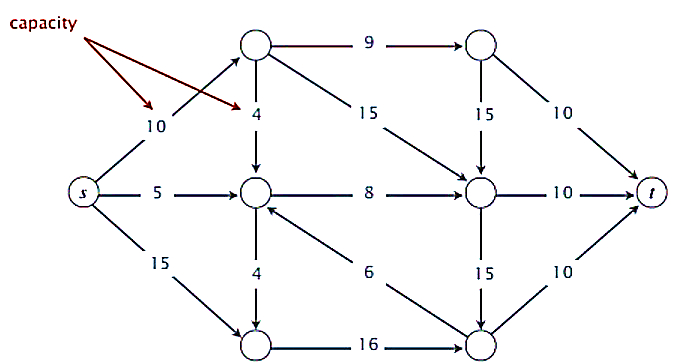
\includegraphics[width=0.65\textwidth]{figures/p3.jpg}}
}
	
%//////////////////////////////////////////////////////////////////////////////////////////////%%4
	\frame{
		\frametitle{A Cache Maintainence Problem}
	\begin{definition}
		A \ccp{cache} is a faster store device than memory which is used to reduce the times of access to memory.

		A \ccp{cache miss} is that when a data item \ccp{d} is requested, \ccp{d} is not in cache. 
	\end{definition}\pause

	\begin{definition}
		We have a set U of \ccp{n} pieces of data stored in main memory and 
		a cache which can hold \ccp{k (k<n)} items.
		Given a visiting sequence of data items \ccp{D ($d_1, d_2, d_3 ... d_m$)} from \ccp{U},
		\ccb{a eviction schedule} to determain which items should be evicted from the cache at which points 
		in the sequence. 
    \end{definition}\pause\bigskip

	}
	%%%//////////////////////////////////////////////////////////////////////////////////////////////%%5


	\frame{
		\frametitle{Cache Maintainence Problem}
		\begin{definition}
			We have a set U of \ccp{n} pieces of data stored in main memory and 
			a cache which can hold \ccp{k (k<n)} items.
			Given a visiting sequence of data items \ccp{D ($d_1, d_2, d_3 ... d_m$)} from \ccp{U},
			\ccb{a eviction schedule} to determain which items should be evicted from the cache at which points 
			in the sequence. 
		\end{definition}
		\vspace{5mm}
		\centerline{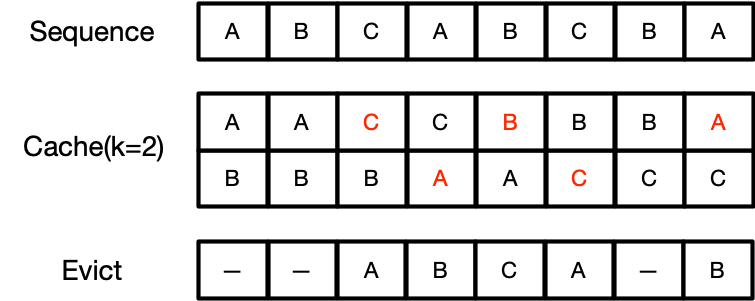
\includegraphics[width=0.7\textwidth]{wsw-pic/cmp.png}}
	}
	%%//////////////////////////////////////////////////////////////////////////////////////////////%%6

	\frame{
		\frametitle{Cache Maintainence Problem}
		
		\cco{Cache Maintainence Problem.} 
		Find an eviction schedule which makes the least number of cache misses.\bigskip\bigskip

		\centerline{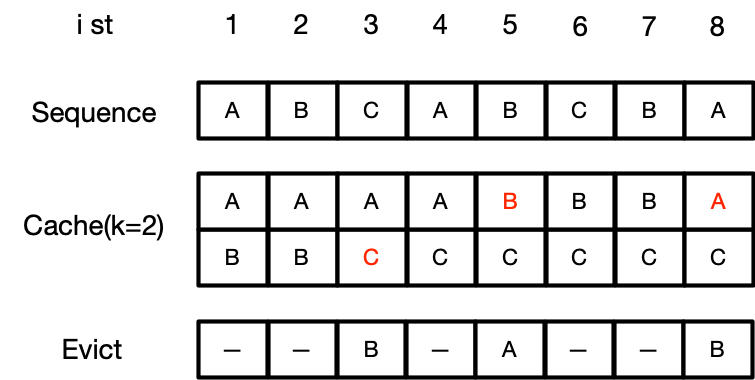
\includegraphics[width=0.6\textwidth]{wsw-pic/bestsche.png}}
	}

	
	%%//////////////////////////////////////////////////////////////////////////////////////////////%%7
	\frame{
		\frametitle{Cache Maintainence Problem}
		\begin{definition}
			A \ccp{Cache Maintainence Problem} can be divided into to different cases:
			\begin{itemize}
				\item \ccb{case one}: the eviction schedule are able to know the coming sequence.
				\item \ccb{case two}: the eviction schedule has to determine without knowledge of what’s coming in the future.
			\end{itemize}
		\end{definition}
		\bigskip
	}
	%%//////////////////////////////////////////////////////////////////////////////////////////////%%7

\section{Farthest-in-Future Algorithm}

	%%//////////////////////////////////////////////////////////////////////////////////////////////%%12
	\frame{
		\frametitle{Farthest-in-Future Algorithm}
		\ccp{Farthest-in-Future Algorithm}
		\vspace{-4mm}
		\begin{itemize}
				\item It is the optimal solution 
						in \ccb{case one} of \ccp{Cache Maintainence Problem}
				\item It is a kind of greedy algorithm.
				\item It is proposed by Les Belady in 1960s
		\end{itemize}\vspace{5mm}
	}
	%
	%%//////////////////////////////////////////////////////////////////////////////////////////////%%13

	\frame{
		\frametitle{Farthest-in-Future Algorithm}
		\ccp{Farthest-in-Future Algorithm.}
		\vspace{-4mm}
		\begin{itemize}
			\item  When \ccb{$d_i$} is in the cache, evict nothing
			\item  When \ccb{$d_i$} is not in the cache and needs to be brought into the cache evict the item that 
			is needed the farthest into the future

		\end{itemize}\vspace{5mm}
		
	}
	%
	%%%%//////////////////////////////////////////////////////////////////////////////////////////////%%14
	%

	\frame{
		\frametitle{Farthest-in-Future Algorithm}
		\ccp{Farthest-in-Future Algorithm.}
		\vspace{-4mm}
		\begin{itemize}
			\item Cache initialize with two item \ccp{A} and \ccp{B}
			\item In step 1 and step 2, data requested are already in cache, no eviction occurs
			\ccg{ \item In step 3, item C is requested but not in the cache. C is brought to cache from memory.
				To make room for C, algorithm evict Item B which is needed the farthest into the future}
			\ccg{ \item In step 4,  item A is already in cache, no eviction occurs}
			\ccg{ \item In step 5,  Item A is evicted for Item B}
			\ccg{ \item In step 6 and step 7,  data requested are already in cache, no eviction occurs}
			\ccg{ \item In step 8,  Item C is evicted for Item A}
		\end{itemize}
		\vspace{4mm}
		\centerline{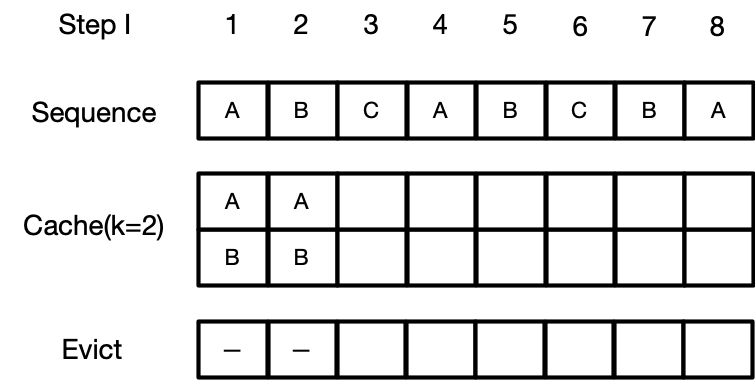
\includegraphics[width=0.52\textwidth]{wsw-pic/ff1}}
	}
	%
	%%%//////////////////////////////////////////////////////////////////////////////////////////////%%15
	\frame{
		\frametitle{Farthest-in-Future Algorithm}
		\ccp{Farthest-in-Future Algorithm.}
		\vspace{-4mm}
		\begin{itemize}
			\ccg{\item Cache initialize with two item A and B}
			\ccg{\item In step 1 and step 2, data requested are already in cache, no eviction occurs}
			\item In step 3, item \ccp{C} is requested but not in the cache. \ccp{C} is brought to cache from memory.
				To make room for \ccp{C}, algorithm evict Item \ccp{B} which is needed the farthest into the future
			\ccg{ \item In step 4,  item A is already in cache, no eviction occurs}
			\ccg{ \item In step 5,  Item A is evicted for Item B}
			\ccg{ \item In step 6 and step 7,  data requested are already in cache, no eviction occurs}
			\ccg{ \item In step 8,  Item C is evicted for Item A}
		\end{itemize}
		\vspace{4mm}
		\centerline{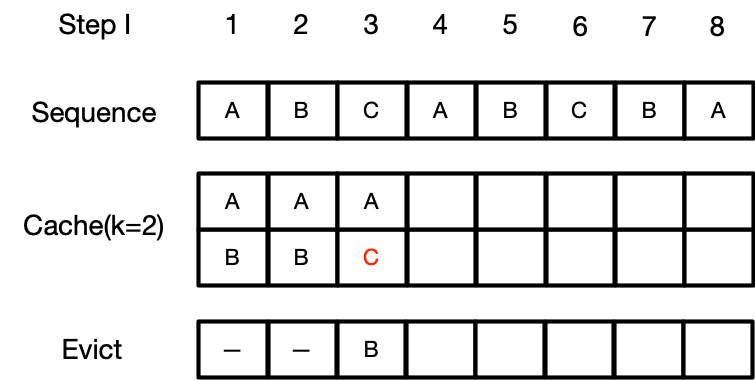
\includegraphics[width=0.52\textwidth]{wsw-pic/ff2}}
	}
%%%%//////////////////////////////////////////////////////////////////////////////////////////////%%19
	\frame{
		\frametitle{Farthest-in-Future Algorithm}
		\ccp{Farthest-in-Future Algorithm.}
		\vspace{-4mm}
		\begin{itemize}
			\ccg{\item Cache initialize with two item A and B}
			\ccg{\item In step 1 and step 2, data requested are already in cache, no eviction occurs}
			\ccg{\item In step 3, item C is requested but not in the cache. C is brought to cache from memory.
				To make room for C, algorithm evict Item B which is needed the farthest into the future}
			\item In step 4,  item \ccp{A} is already in cache, no eviction occurs
			\ccg{ \item In step 5,  Item A is evicted for Item B}
			\ccg{ \item In step 6 and step 7,  data requested are already in cache, no eviction occurs}
			\ccg{ \item In step 8,  Item C is evicted for Item A}
		\end{itemize}
		\vspace{4mm}
		\centerline{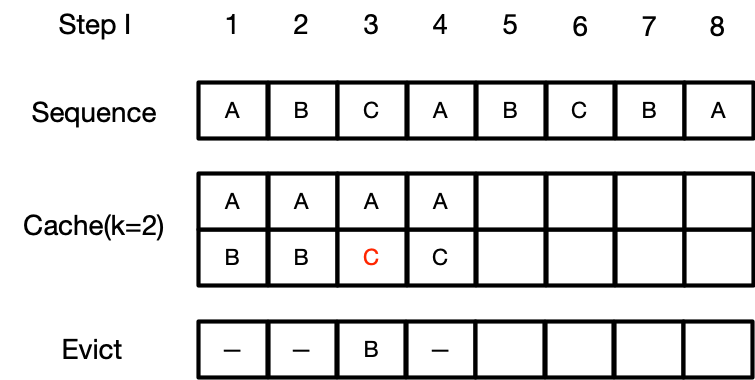
\includegraphics[width=0.52\textwidth]{wsw-pic/ff3}}
	}

%%%%//////////////////////////////////////////////////////////////////////////////////////////////%%19

	\frame{
		\frametitle{Farthest-in-Future Algorithm}
		\ccp{Farthest-in-Future Algorithm.}
		\vspace{-4mm}
		\begin{itemize}
			\ccg{\item Cache initialize with two item A and B}
			\ccg{\item In step 1 and step 2, data requested are already in cache, no eviction occurs}
			\ccg{\item In step 3, item C is requested but not in the cache. C is brought to cache from memory
				To make room for C, algorithm evict Item B which is needed the farthest into the future}
			\ccg{ \item In step 4,  item A is already in cache, no eviction occurs}
			\item In step 5,  Item \ccp{A} is evicted for Item \ccp{B}
			\ccg{ \item In step 6 and step 7,  data requested are already in cache, no eviction occurs}
			\ccg{ \item In step 8,  Item C is evicted for Item A}
		\end{itemize}
		\vspace{4mm}
		\centerline{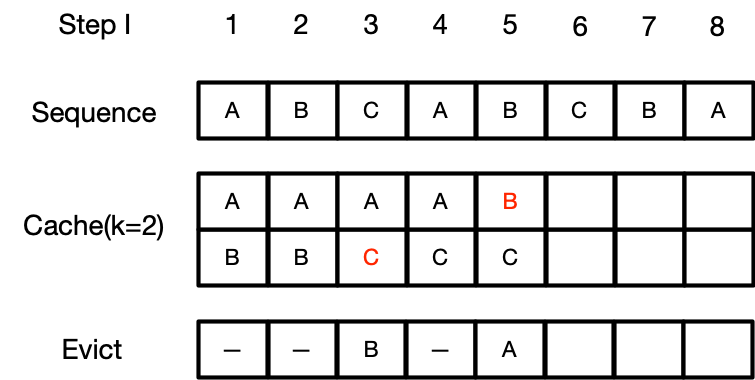
\includegraphics[width=0.52\textwidth]{wsw-pic/ff4}}
	}
%%%%//////////////////////////////////////////////////////////////////////////////////////////////%%19
	
	\frame{
		\frametitle{Farthest-in-Future Algorithm}
		\ccp{Farthest-in-Future Algorithm.}
		\vspace{-4mm}
		\begin{itemize}
			\ccg{\item Cache initialize with two item A and B}
			\ccg{\item In step 1 and step 2, data requested are already in cache, no eviction occurs}
			\ccg{\item In step 3, item C is requested but not in the cache. C is brought to cache from memory
				To make room for C, algorithm evict Item B which is needed the farthest into the future}
			\ccg{ \item In step 4,  item A is already in cache, no eviction occurs}
			\ccg{\item In step 5,  Item A is evicted for Item B}
			\item In step 6 and step 7,  data requested are already in cache, no eviction occurs
			\ccg{ \item In step 8,  Item C is evicted for Item A}
		\end{itemize}
		\vspace{4mm}
		\centerline{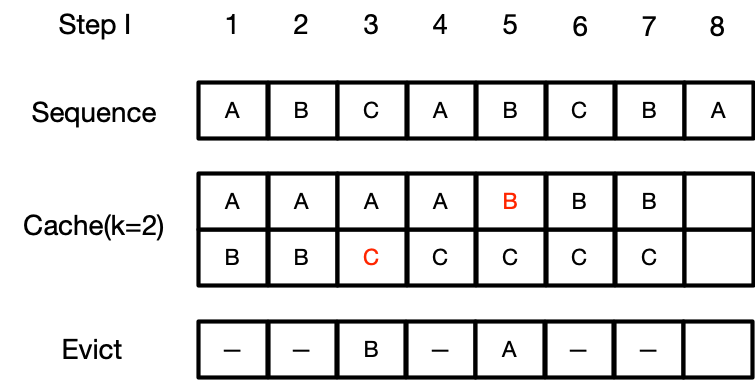
\includegraphics[width=0.52\textwidth]{wsw-pic/ff5}}
	}
%%%%//////////////////////////////////////////////////////////////////////////////////////////////%%19
	\frame{
		\frametitle{Farthest-in-Future Algorithm}
		\ccp{Farthest-in-Future Algorithm.}
		\vspace{-4mm}
		\begin{itemize}
			\ccg{\item Cache initialize with two item A and B}
			\ccg{\item In step 1 and step 2, data requested are already in cache, no eviction occurs}
			\ccg{\item In step 3, item C is requested but not in the cache. C is brought to cache from memory.
				To make room for C, algorithm evict Item B which is needed the farthest into the future}
			\ccg{ \item In step 4,  item A is already in cache, no eviction occurs}
			\ccg{\item In step 5,  Item A is evicted for Item B}
			\ccg{\item In step 6 and step 7,  data requested are already in cache, no eviction occurs}
			\item In step 8,  Item \ccp{C} is evicted for Item \ccp{A}
		\end{itemize}
		\vspace{4mm}
		\centerline{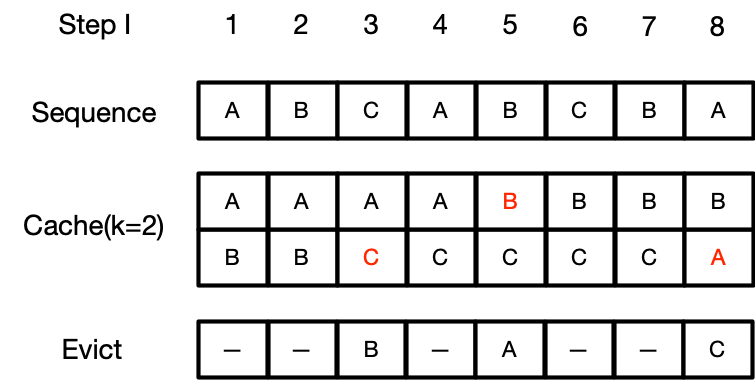
\includegraphics[width=0.52\textwidth]{wsw-pic/ff6}}
	}
	%%%%//////////////////////////////////////////////////////////////////////////////////////////////%%19

	\frame{
		\frametitle{Reduced Schedule}
		\begin{definition}
			An eviction schedule is \ccp{reduced} if it fetches an item x only when it is accessed
		\end{definition}
		\vspace{5mm}
		\centerline{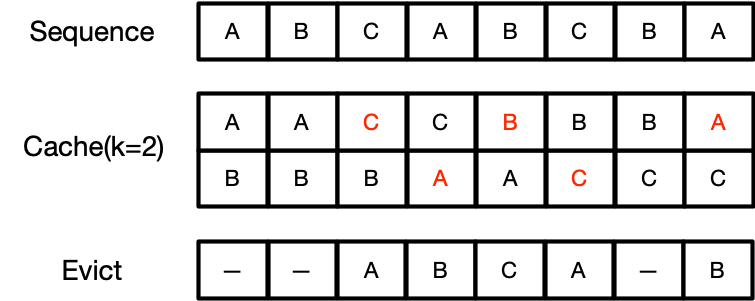
\includegraphics[width=0.7\textwidth]{wsw-pic/cmp.png}}	
	}
	%%%%//////////////////////////////////////////////////////////////////////////////////////////////%%20
	\frame{
		\frametitle{Reduced Schedule}
		\ccr{schedule(a)} is reduced 

		It fetches item \ccp{C} in step 3  when \ccp{C} is accessed

		\ccr{schedule(b)} is not reduced 

		It fetches item \ccp{C} in step 2  but \ccp{C} is not requested 

		\vspace{15mm}
		\centerline{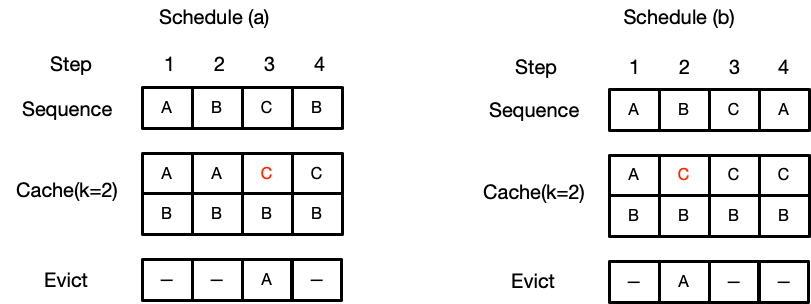
\includegraphics[width=0.9\textwidth]{wsw-pic/twosche.png}}	
	}

	\frame{
		\frametitle{Reduced Schedule}
		\begin{lemma}
			For any non-reduced schedule S, we are able to construct a reduced schedule $\bar{S}$,
			which is the reduction of S and brings in at most as many items as the schedule S.
		\end{lemma}

		\vspace{15mm}
		\centerline{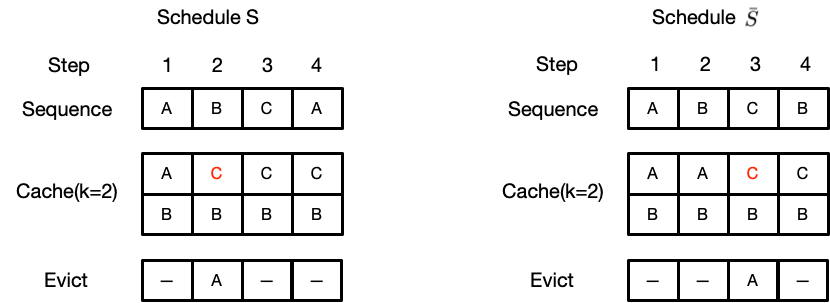
\includegraphics[width=0.9\textwidth]{wsw-pic/twosche2.png}}	
	}

	%%%%//////////////////////////////////////////////////////////////////////////////////////////////%%21

\frame{
	\frametitle{Reduced Schedule}
	\begin{lemma}
		For any non-reduced schedule S, we are able to construct a reduced schedule $\bar{S}$,
		which is the reduction of S and brings in at most as many items as the schedule S.
	\end{lemma}

	\begin{proof}
		We can construct using the following steps:
		\begin{itemize}
			\item In step i, when item \ccp{d} has not been requested, but S brings item \ccp{d} into the cache and evict item \ccp{e}.
				  $\bar{S}$ leaves item d in memory.
			\item In step j, when item d is requested. $\bar{S}$ brings item \ccp{d} into the cache and evict item \ccp{e}.
			\item Otherwise, $\bar{S}$ do the same thing as S
		\end{itemize}
		The cache miss incurred by $\bar{S}$ in step j can be charged to the earlier cache operation 
		performed by S in step i, when it brought in d.
	\end{proof}

	}
%%%%//////////////////////////////////////////////////////////////////////////////////////////////%%45
	\frame{
		\frametitle{Prove that Farthest-in-Future Algorithm is optimal}
		\begin{definition}
			Let \ccp{D} denote the arbitrary sequence of memory references. 
			Let $S_{FF}$ denote the schedule produced by Farthest-in-Future. 
			Let $S_∗$ denote a schedule that incurs the minimum possible number of misses.
		\end{definition}
		
		\begin{lemma}
			For a number j, Let S be a reduced schedule that makes the same eviction decisions as $S_{FF}$
			through the first j items in the sequence. 
			There exist a reduced schedule S' that makes the same eviction decisions as  $S_{FF}$ through the first j + 1 items.
			S' incurs no more misses than S does.
		\end{lemma}
	}
%%%%//////////////////////////////////////////////////////////////////////////////////////////////%%46
\frame{
	\frametitle{Prove that Farthest-in-Future Algorithm is optimal}
	\ccr{Note}

	Suppose item d = $d_{j+1}$ is requested at step (j+1). Since schedule S and S'
	make the same eviction decisions as $S_{FF}$ through the first j steps. 
	They have the same cache contents, before d is requested.


	\vspace{5mm}
	\centerline{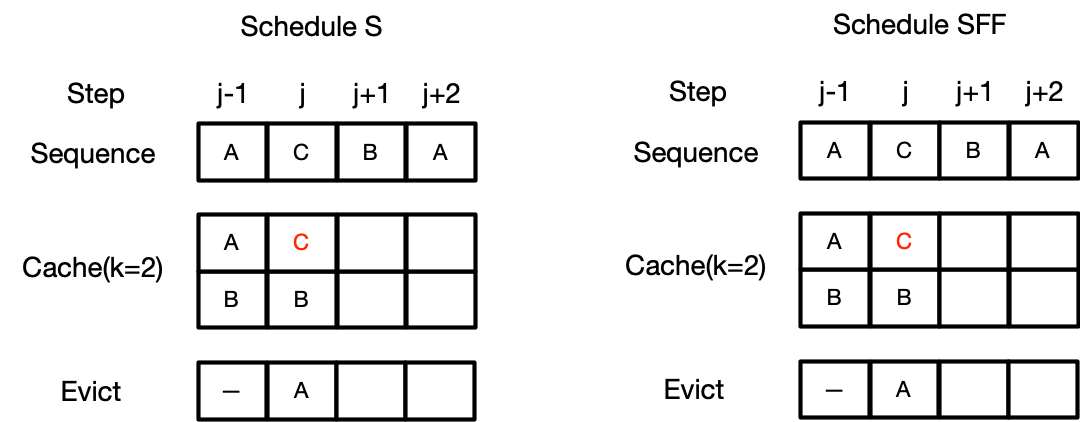
\includegraphics[width=0.9\textwidth]{wsw-pic/sff1.png}}	
}

\frame{
	\frametitle{Prove that Farthest-in-Future Algorithm is optimal}

	\begin{proof}
		\ccr{Case one}: \ccp{d is in the cache for both}
		
		In step j+1, S makes the same eviction decisions(evict nothing) as $S_{FF}$.
		Hence we can construct S' = S in this case
	\end{proof}


	\vspace{5mm}
	\centerline{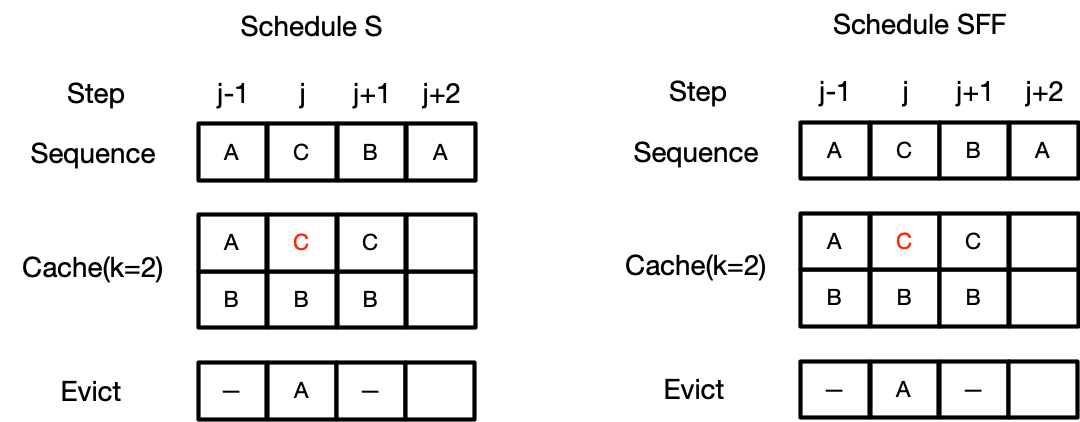
\includegraphics[width=0.9\textwidth]{wsw-pic/sff2.png}}	
}
%%%%//////////////////////////////////////////////////////////////////////////////////////////////%%47

\frame{
	\frametitle{Prove that Farthest-in-Future Algorithm is optimal}

	\begin{proof}
		\ccr{Case two}: \ccp{d is not in the cache for both and S and $S_{FF}$ both evict the same item to make room for d}
		
		In step j+1, both S and $S_{FF}$ evict the same item and bring \ccp{d} into the cache.
		Hence we can construct S' = S in this case
	\end{proof}


	\vspace{5mm}
	\centerline{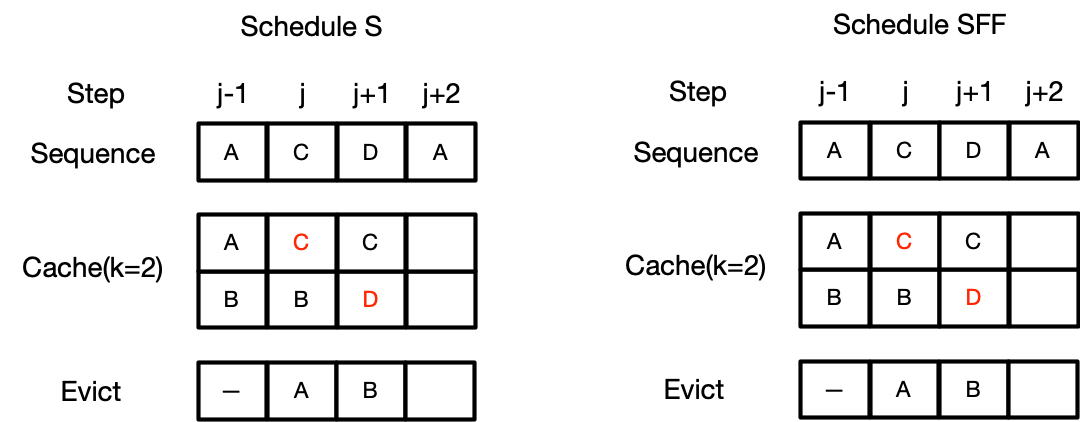
\includegraphics[width=0.9\textwidth]{wsw-pic/sff3.png}}	
}
%%%%//////////////////////////////////////////////////////////////////////////////////////////////%%48

\frame{
	\frametitle{Prove that Farthest-in-Future Algorithm is optimal}

	\begin{proof}
		\ccr{Case three}: \ccp{d is not in the cache for both and S and $S_{FF}$ evict the different item to make room for d. 
								For S, item f is evicted. For $S_{FF}$ , item e is evicted. e $\neq$ f}
		
		S' is supposed to evict e rather than f at step j+1. 
		To ensure that S' incurs no more misses than S in the furture, 
		S' should try to get its cache back to the same state as S as quickly as possible,
		so as to having it behave like S later.
	\end{proof}

	\vspace{5mm}
	\centerline{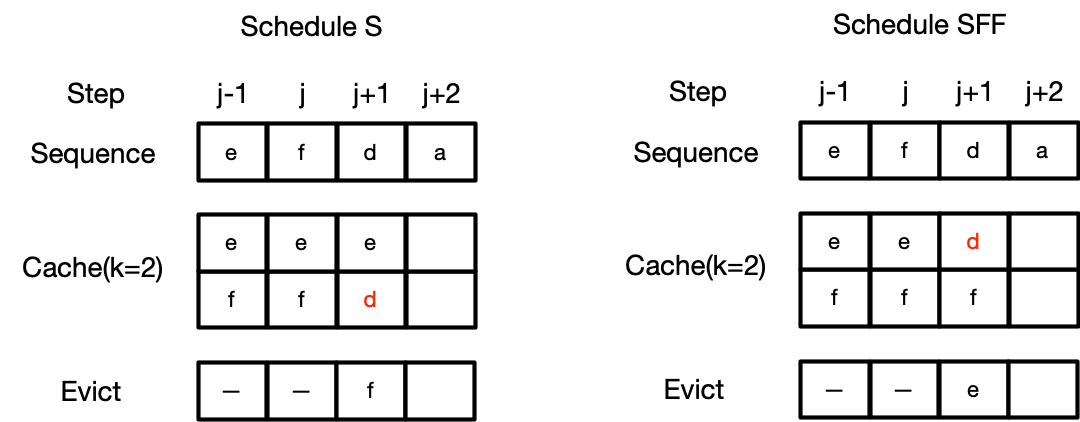
\includegraphics[width=0.9\textwidth]{wsw-pic/sff4.png}}	
}

%%%%//////////////////////////////////////////////////////////////////////////////////////////////%%48
	\frame{
		\frametitle{Prove that Farthest-in-Future Algorithm is optimal}

		\begin{proof}
			\ccr{Case three}: \ccp{For S, item f is evicted. For $S_{FF}$ , item e is evicted. e $\neq$ f}
			
			from request j+2 onward, S‘ behaves exactly like S  until one of the following things happens for the first time
			\begin{itemize}
				\item 
				(a) An item g is requested and g $\neq$ e and S evicts e to make room for g. 
				In this case we can have S' evict f instead of e.
				Then, S and S' have the same cache state. 
				Hence, S' incurs no more misses than S in this case.
			\end{itemize}
		\end{proof}
		\vspace{1mm}
		\centerline{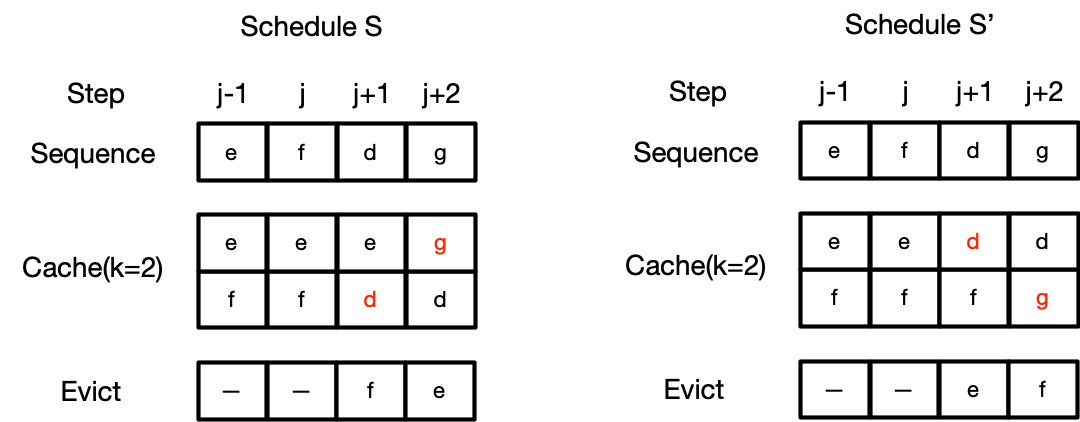
\includegraphics[width=0.9\textwidth]{wsw-pic/sff5.png}}	
	}
%%%%//////////////////////////////////////////////////////////////////////////////////////////////%%48

	\frame{
		\frametitle{Prove that Farthest-in-Future Algorithm is optimal}

		\begin{proof}
			\ccr{Case three}: \ccp{For S, item f is evicted. For $S_{FF}$ , item e is evicted. e $\neq$ f}
			
			from request j+2 onward, S‘ behaves exactly like S  until one of the following things happens for the first time
			\begin{itemize}
				\item 
				(b) The item f is requested and S evicts an item $e'$ and  $e' = e$, 
				then schedule $S'$ can reach the same cache state with $S$ after this step
				by simply accessing f from the cache. Then $S$ and $S'$ will be same after this step.
			\end{itemize}
			
		\end{proof}

		\vspace{1mm}
		\centerline{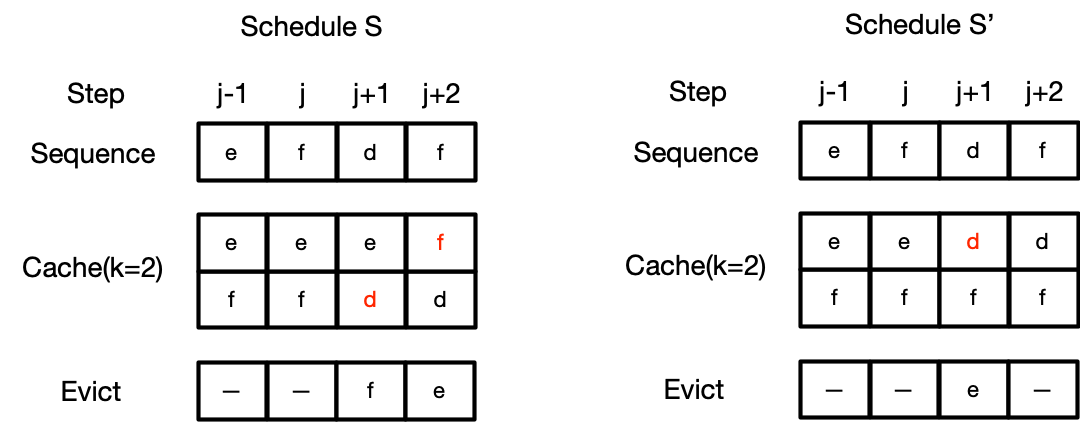
\includegraphics[width=0.9\textwidth]{wsw-pic/sff6.png}}	
	}
%%%%//////////////////////////////////////////////////////////////////////////////////////////////%%48

	\frame{
		\frametitle{Prove that Farthest-in-Future Algorithm is optimal}

		\begin{proof}
			\ccr{Case three}: \ccp{For S, item f is evicted. For $S_{FF}$ , item e is evicted. e $\neq$ f}
			
			from request j+2 onward, S‘ behaves exactly like S  until one of the following things happens for the first time
			\begin{itemize}
				\item (c) 
				The item f is requested and S evicts an item $e'$ and  $e' \neq e$, 
				then $S'$ can reach the same cache state with $S$ by evicting $e'$ and bringing 
				$e$ back to the cache.
				$S'$ incurs no more misses than $S$ does in this case
			\end{itemize}
		\end{proof}

		\vspace{1mm}
		\centerline{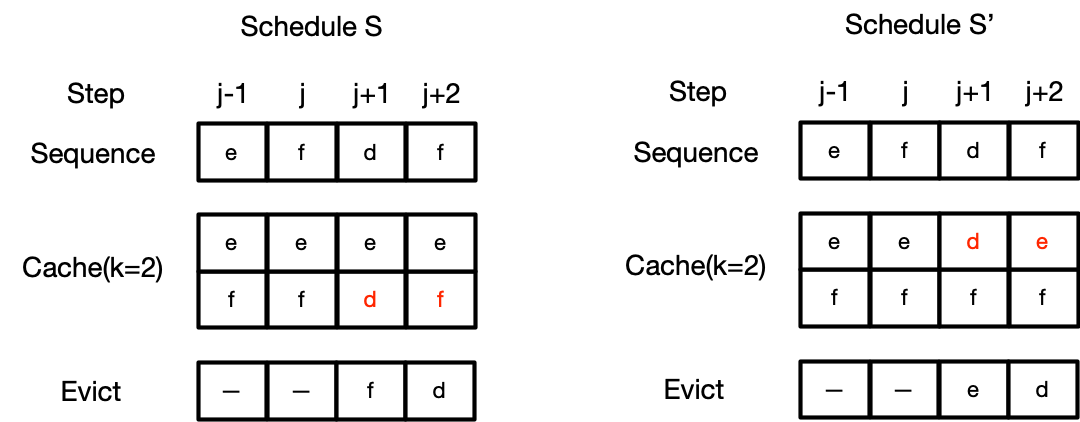
\includegraphics[width=0.9\textwidth]{wsw-pic/sff7.png}}	
	}
%%%%//////////////////////////////////////////////////////////////////////////////////////////////%%48

	\frame{
		\frametitle{Prove that Farthest-in-Future Algorithm is optimal}

		\begin{proof}
			\ccr{Case three}: \ccp{For S, item f is evicted. For $S_{FF}$ , item e is evicted. e $\neq$ f}
			
			from request j+2 onward, S‘ behaves exactly like S  until one of the following things happens for the first time
			\begin{itemize}
				\item (d) The item e is requested. This case will not happen before \ccp{case(b)}
				\item (e) In other condition, We can have S' do the same thing as S and $S'$ incurs no more misses than $S$ does in this case.
			\end{itemize}		
			
		\end{proof}	
	}
%%%%//////////////////////////////////////////////////////////////////////////////////////////////%%48
	\frame{
		\frametitle{Prove that Farthest-in-Future Algorithm is optimal}

		\begin{definition}
			Let \ccp{D} denote the arbitrary sequence of memory references. 
			Let $S_{FF}$ denote the schedule produced by Farthest-in-Future. 
			Let $S_∗$ denote a schedule that incurs the minimum possible number of misses.
		\end{definition}

		\begin{theorem}
			$S_{FF}$ incurs no more misses than any other schedule $S*$ and hence is optimal
		\end{theorem}
	}
%%%%//////////////////////////////////////////////////////////////////////////////////////////////%%48
\frame{
	\frametitle{Prove that Farthest-in-Future Algorithm is optimal}
	\begin{proof}
		We prove this claim by transforming $S^*$ to $S_{FF}$ with no more missed.
		\begin{enumerate}
			\item  we can set $S_0 = S^*$ because $S^*$ and $S_{FF}$ have the same cache state before the first
			item access.
			\item  According to lemma above, there exits a reduced schedule $S_1$ that makes the same eviction decisions as $S_{FF}$ 
			through the first j + 1 items and incurs no more misses than $S_0$ does. we are able to construct $S_1$ 
			\item  We continue applying lemma above inductively for j = 1, 2, 3, ... , m, producing schedules $S_j$ 
			that agree with $S_{FF}$ through the first j steps. 
			As $S_{j+1}$ incurs no more misses than $S_{j}$ for each j, $S_m$ also incurs no more misses than $S^*$
			\item  As we can have $S_m = S_{FF}$ by the definition, 
			it is proved that $S_{FF}$ incurs no more misses than $S^*$ and hence is optimal.
		\end{enumerate}  
	\end{proof}	
}
%%%%//////////////////////////////////////////////////////////////////////////////////////////////%%48

	\frame{
		\frametitle{Conclusion in this section}


		\ccr{Conclusion}: 
			
		\begin{itemize}
			\item  Introduce a Farthest-in-Future Algorithm which is used to solve Caching problem given request sequence
			\item  Introduce the reduced schedule
			\item  Prove that Farthest-in-Future Algorithm is optimal
		\end{itemize}		
		
	}
%%%%//////////////////////////////////////////////////////////////////////////////////////////////%%48

\section{Marking Algorithms}

%%%%//////////////////////////////////////////////////////////////////////////////////////////////%%48
	%%
	\frame{
		\frametitle{Marking Algorithms}
		\begin{itemize}
			\item solve the problem in Case two (The eviction schedule has to determine without knowledge of what’s coming in the future)
			\item it is a a class of algorithms rather than a single specific algorithm
		\end{itemize}

		
		\vspace{8mm}
		\centerline{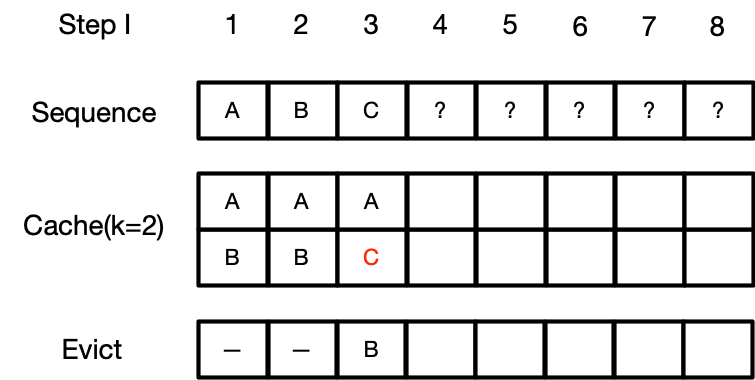
\includegraphics[width=0.7\textwidth]{wsw-pic/marking.png}}

	}
%%//////////////////////////////////////////////////////////////////////////////////////////////%%58
	\frame{
		\frametitle{Marking Algorithms}
		\begin{exampleblock}{}
			\begin{algorithm}[H]
				\SetKwData{x}{x}\SetKwData{y}{y}\SetKwData{z}{z}
				\SetKwFunction{CS}{\sc Marking Schdule}\SetKwFunction{Return}{\sc Return}\SetKwFunction{Init}{\sc Initialize}
				\SetKwFunction{Up}{\sc Update}\SetKwFunction{Au}{\sc Augment}\SetKwFunction{BFS}{\sc BFS}
				\SetKwInOut{Input}{input}\SetKwInOut{Output}{output}
			\CS{Sequence}
			\BlankLine
			Unmark all items

			\For{each item $s \in Sequence$}{
				
				Mark s

				\If{$s$ is not in cache}{
					evict nothing
				}\Else{
					\If{all items currently in the cache are marked}{
						Declare the phase over

						Processing of s is deferred to start of next phase
					}\Else{
						Evict an unmarked item from the cache
					}
				}
			}
			\end{algorithm}
			\end{exampleblock}
	}
%%//////////////////////////////////////////////////////////////////////////////////////////////%%58
\frame{
	\frametitle{Marking Algorithms}
	\begin{definition}
		To make it easy to analysis.
		\begin{enumerate}
			\item Add a Phase 0 that takes place before the first phase. In phase 0, all the items initially in the cache are requested once.
			\item Add a epilogue in final Phase r, in which every item currently in the cache of the optimal algorithm is requested twice in roundrobin fashion
		  \end{enumerate} 
	\end{definition}
	\vspace{4mm}
	\centerline{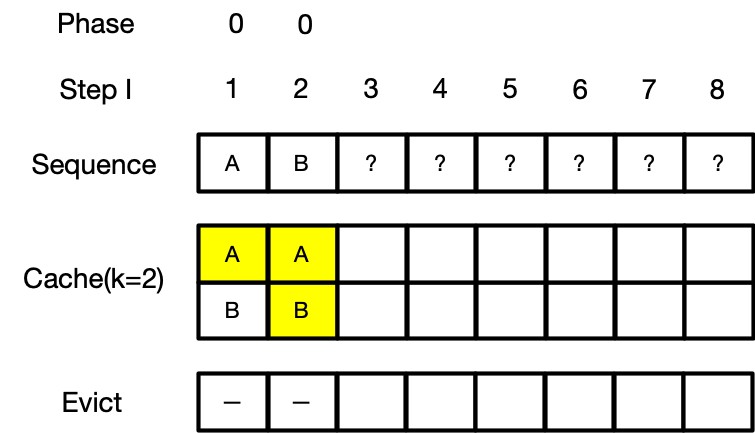
\includegraphics[width=0.6\textwidth]{wsw-pic/markp0.png}}
}
%%//////////////////////////////////////////////////////////////////////////////////////////////%%58
\frame{
	\frametitle{Marking Algorithms}
	\begin{exampleblock}
		A
		According to Marking Algorithm
		\begin{enumerate}
			\item In step 3, C is not in cache and all cache items are marked, as a aresult phase 0 is over and phase 1 begins.
				  Item C is marked
			\item In step 4, C is in the cache and marked, so evict nothing.
		  \end{enumerate} 
	\end{exampleblock}
	\vspace{4mm}
	\centerline{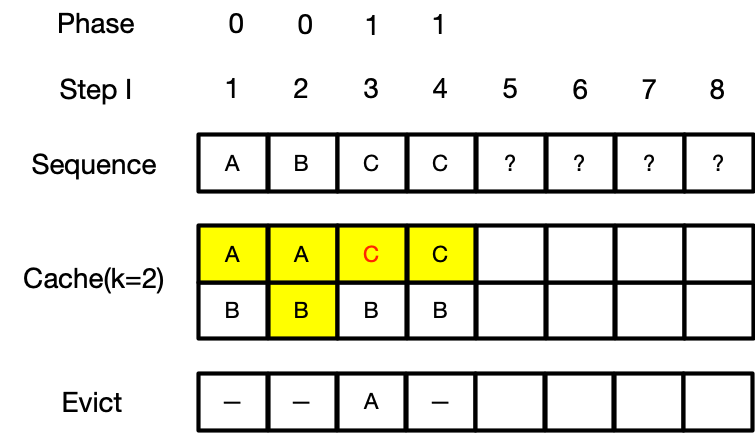
\includegraphics[width=0.6\textwidth]{wsw-pic/markp1.png}}
}
%%//////////////////////////////////////////////////////////////////////////////////////////////%%58
\frame{
	\frametitle{Marking Algorithms}
	\begin{exampleblock}
		A
		According to Marking Algorithm
		\begin{enumerate}
			\item In step 5, B is in cache but not marked. So, evict nothing and mark B.
		  \end{enumerate} 
	\end{exampleblock}
	\vspace{4mm}
	\centerline{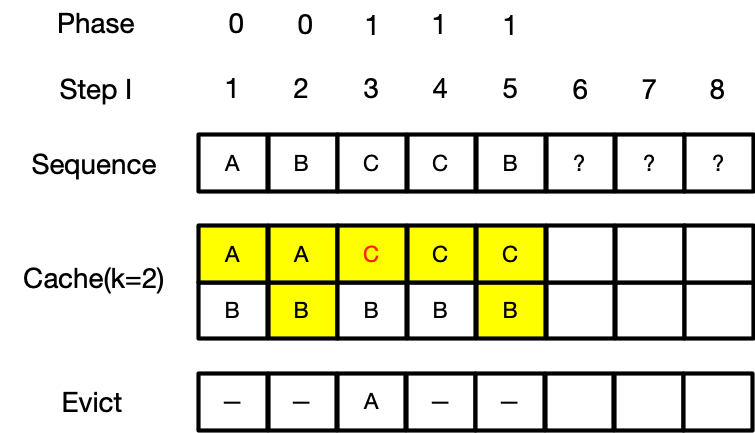
\includegraphics[width=0.6\textwidth]{wsw-pic/markp2.png}}
}
%%//////////////////////////////////////////////////////////////////////////////////////////////%%58
\frame{
	\frametitle{Marking Algorithms}
	\begin{exampleblock}
		A
		According to Marking Algorithm
		\begin{enumerate}
			\item In step 6, A is in not cache and all cache items are marked. 
				  So, unmark all item in cache and begin a new phase.
				  Then evcit an item to make room for A. Mark A
		  \end{enumerate} 
	\end{exampleblock}
	\vspace{4mm}
	\centerline{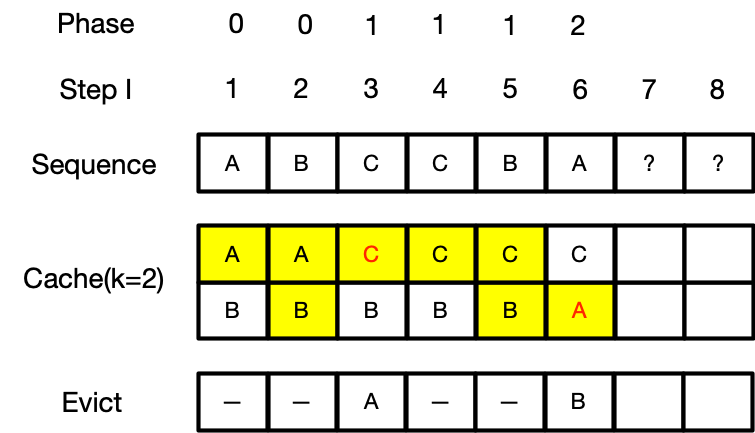
\includegraphics[width=0.6\textwidth]{wsw-pic/markp3.png}}
}
%%//////////////////////////////////////////////////////////////////////////////////////////////%%58
\frame{
	\frametitle{Marking Algorithms}
	\begin{exampleblock}
		A
		Suppose phase 2 is the last phase r (r = 2).
		According to the definition.

		\begin{enumerate}
			\item In step 7 and 8, we request all item in cache twice in roundrobin fashion
		  \end{enumerate} 
	\end{exampleblock}
	\vspace{4mm}
	\centerline{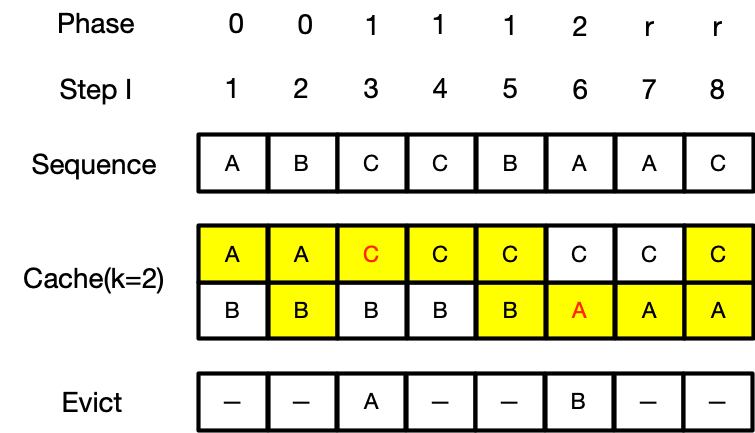
\includegraphics[width=0.6\textwidth]{wsw-pic/markp4.png}}
}
%%//////////////////////////////////////////////////////////////////////////////////////////////%%58
\frame{
	\frametitle{Analysis of Marking Algorithms}
	\ccp{Marking Algorithms}

	\begin{itemize}
		\item it is a class of algorithms rather than a single specific algorithm, because it does not specify which unmarked item should be selected
		\item It is cleared that any Marking Algorithm incurs more cache misses than $S_{FF}$
		\item Missed occurs under 2 cases.
			\begin{itemize}
				\item case a : In the recent past, the request sequence has contained more than k distinct items
				\item case b : In the recent past, the request sequence has come exclusively from a set of at most k items
			\end{itemize}
			In Case a, cache misses cannot be improved.

			In Case b, a marking algorithm is possiable to lower the missed caused  and we can analayze the algorithm according to the baseline(optimal)
	\end{itemize}
}
%%//////////////////////////////////////////////////////////////////////////////////////////////%%58
\frame{
	\frametitle{Analysis of Marking Algorithms}
	\ccp{Marking Algorithms}
	\begin{definition}
		$f(\delta)$ to denote the minimum number of misses it is possible to make on sequence $\delta$.
		$f(\delta)$ is the number of misses achieved by the optimal Farthest-in-Future policy.
	\end{definition}
}
%%//////////////////////////////////////////////////////////////////////////////////////////////%%58
\frame{
	\frametitle{Analysis of Marking Algorithms}
	\ccp{Marking Algorithms}
	\begin{claim}
		In each phase, $\delta$ contains accesses to exactly k distinct items.
		The subsequent phase begins with an access to a different $(k + 1)^{st}$ item.
	  \end{claim}
	  
	  \begin{proof}
		This claim can be proved by pigeonhole principle. As we have only k unmarked slot for k different item, 
		there is no extra unmarked slot for the $(k+1)^{st}$ item, and thus the subsequent phase begins with the $(k+1)^{st}$ item.
	  \end{proof}
}
%%//////////////////////////////////////////////////////////////////////////////////////////////%%58
\frame{
	\frametitle{Analysis of Marking Algorithms}
	\ccp{Marking Algorithms}
	\begin{claim} 
		The marking algorithm incurs at most k misses per phase, for a total of at most kr misses over all r phases.
	\end{claim}
	  
	\begin{proof}
		As the subsequent phase begins with an access to a different $(k + 1)^{st}$ item, there  musy exactly be different k items being 
		accessed during the phase.  Hence the algorithm incures at most k misses per phase, for a total of at most kr misses over all r phases.
	\end{proof}
}
%%//////////////////////////////////////////////////////////////////////////////////////////////%%58
\frame{
	\frametitle{Analysis of Marking Algorithms}
	\ccp{Marking Algorithms}
	\begin{claim} 
		The optimum incurs at least r−1 misses. In other words, $f(\delta) \geq {r-1} $
	  \end{claim}
	  
	  \begin{proof}
		Consider any phase but the first one and look at the situation when the first item is accessed in any new phase. 
		The first request must cause a miss, otherwise the new phase will not begin. However, the first phase may not cause any miss 
		if all items accessed in phase one have been already in the cache after phase 0. 
		As a result any algorithm incurs at least r−1 misses and  $f(\delta) \geq {r-1}$.
	  
		Then Consider the tight case. Let us look at the situation just after the first access in any phase but the first one. 
		Algorithm above shows that the remainder of the phase will involve accesses to k − 1 other distinct items.
		If those  k − 1 other distinct items have already been in the cache when the last phase is over, 
		then the optimum incurs exactly r − 1 misses.
	  \end{proof}
}
%%//////////////////////////////////////////////////////////////////////////////////////////////%%58
\frame{
	\frametitle{Analysis of Marking Algorithms}
	\ccp{Marking Algorithms}
	\begin{theorem}
		For any marking algorithm, the number of misses it incurs on any sequence $\delta$ is at most $k·f(\delta)+k$.
	\end{theorem}
	  
	\begin{proof}
		This can be proved with the help of Claim above.
		$kr = k(r-1)+r \leq k·f(\delta)+k$
	\end{proof}
}
%%//////////////////////////////////////////////////////////////////////////////////////////////%%58
\section{Least-Recently-Used Algorithm}
%%//////////////////////////////////////////////////////////////////////////////////////////////%%58
\frame{
	\frametitle{LRU Algorithm}
	\ccp{LRU Algorithms}
	\begin{itemize}
		\item LRU Algorithm is a kind of Marking Algorithm
		\item LRU Algorithm is likely to reach the worst case
	\end{itemize}
}	
%%%%//////////////////////////////////////////////////////////////////////////////////////////////%%73
\frame{
	\frametitle{LRU Algorithm}
	\begin{exampleblock}{}
		\begin{algorithm}[H]
			\SetKwData{x}{x}\SetKwData{y}{y}\SetKwData{z}{z}
			\SetKwFunction{CS}{\sc LRU }\SetKwFunction{Return}{\sc Return}\SetKwFunction{Init}{\sc Initialize}
			\SetKwFunction{Up}{\sc Update}\SetKwFunction{Au}{\sc Augment}\SetKwFunction{BFS}{\sc BFS}
			\SetKwInOut{Input}{input}\SetKwInOut{Output}{output}
		\CS{Sequence}
		\BlankLine
		Unmark all items

		\For{each item $s \in Sequence$}{
			
			Mark s

			\If{$s$ is not in cache}{
				evict nothing
			}\Else{
				\If{all items currently in the cache are marked}{
					Declare the phase over

					Processing of s is deferred to start of next phase
				}\Else{
					\ccr{Evict the least recently used item}
				}
			}
		}
		\end{algorithm}
		\end{exampleblock}
}
%%//////////////////////////////////////////////////////////////////////////////////////////////%%58
\frame{
	\frametitle{LRU Algorithm}
	\ccp{LRU Algorithms}
	\begin{claim}
		LRU algorithm is a Marking Algorithm.
	\end{claim}
	\begin{proof}
		At any point in a phase, if there are any unmarked items in the cache, 
		then the least recently used item must be unmarked.
		Hence, LRU is a marking algorithm.
	\end{proof}
}		
%%%%//////////////////////////////////////////////////////////////////////////////////////////////%%73
\frame{
	\frametitle{LRU Algorithm}
	\ccp{LRU Algorithms}
	\begin{example} 
		  There is a request sequence in which k + 1 items are repeatedly requested in a round-robin fashion and 
		our cache have k slot to store items.
	\end{example}
	\vspace{2mm}\centerline{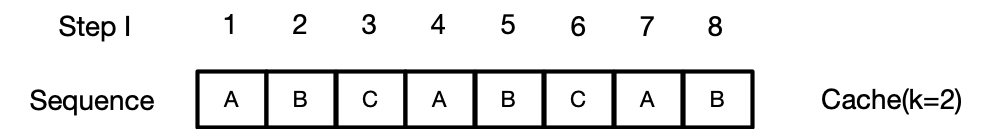
\includegraphics[width=0.6\textwidth]{wsw-pic/worstcase.png}}

	In this example, \ccp{LRU} will evict the item which will be requested in the next step, as a result, misses are incurred on each access.
	
	The \ccp{Farthest-in-Future Algorithm} evcit the item that will be requested farthest in the future,
	and thus the optimal policy incurs only one miss in every k steps. 
	
	So LRU have the worst performance($kf(\delta)$) in this workload.
}
%%%%//////////////////////////////////////////////////////////////////////////////////////////////%%73
\frame{
	\frametitle{LRU Algorithm}
	\begin{example} 
		  There is a request sequence in which k + 1 items are repeatedly requested in a round-robin fashion and 
		our cache have k slot to store items.
	\end{example}
	\ccp{LRU Algorithms}
	\vspace{10mm}
	\centerline{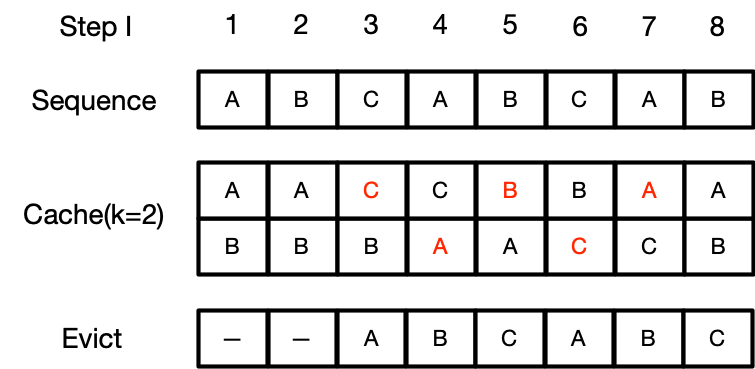
\includegraphics[width=0.6\textwidth]{wsw-pic/lru.png}}
}
%%%%//////////////////////////////////////////////////////////////////////////////////////////////%%73
\frame{
	\frametitle{LRU Algorithm}
	\begin{example}  
		  There is a request sequence in which k + 1 items are repeatedly requested in a round-robin fashion and 
		our cache have k slot to store items.
	\end{example}
	\ccp{Farthest-in-Future Algorithm}
	\vspace{10mm}
	\centerline{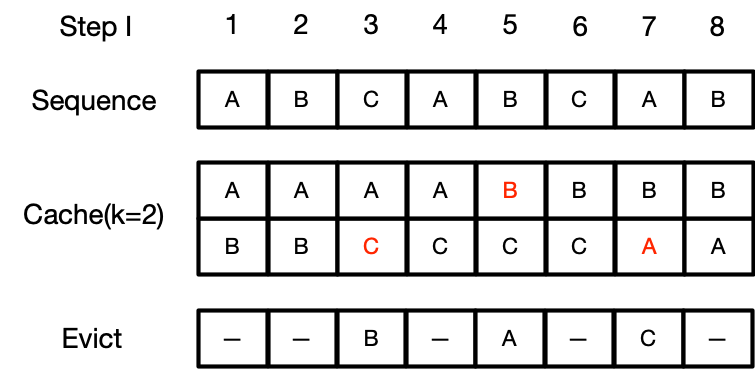
\includegraphics[width=0.6\textwidth]{wsw-pic/sffw.png}}
}			
%%%%//////////////////////////////////////////////////////////////////////////////////////////////%%73
\section{Random Marking Algorithms}
%%//////////////////////////////////////////////////////////////////////////////////////////////%%58
\frame{
	\frametitle{Random Marking Algorithms}
	\begin{exampleblock}{}
		\begin{algorithm}[H]
			\SetKwData{x}{x}\SetKwData{y}{y}\SetKwData{z}{z}
			\SetKwFunction{CS}{\sc LRU }\SetKwFunction{Return}{\sc Return}\SetKwFunction{Init}{\sc Initialize}
			\SetKwFunction{Up}{\sc Update}\SetKwFunction{Au}{\sc Augment}\SetKwFunction{BFS}{\sc BFS}
			\SetKwInOut{Input}{input}\SetKwInOut{Output}{output}
		\CS{Sequence}
		\BlankLine
		Unmark all items

		\For{each item $s \in Sequence$}{
			
			Mark s

			\If{$s$ is not in cache}{
				evict nothing
			}\Else{
				\If{all items currently in the cache are marked}{
					Declare the phase over

					Processing of s is deferred to start of next phase
				}\Else{
					\ccr{Evict an unmarked item chosen uniformly at random from the cache}
				}
			}
		}
		\end{algorithm}
		\end{exampleblock}
}	
%%%%//////////////////////////////////////////////////////////////////////////////////////////////%%73
\frame{
	\frametitle{Random Marking Algorithms}
	\begin{definition}
		The phase begins with all items unmarked, and it contains accesses to \ccp{k} distinct items.
		Each of these items goes from unmarked to marked the first time it is accessed.
		The unmarked items in the middle of a phase are classfied into two further categories:
		\begin{enumerate}
		  \item fresh : an unmarked item was not marked in the previous phase.
		  \item stale : an unmarked item was marked in the previous phase.
		\end{enumerate}
	  
		Among these \ccp{k} accesses to unmarked items in phase \ccp{j}, 
		let \ccp{$c_j$} denote the number of these that are to fresh items.
	\end{definition}
}
%%%%//////////////////////////////////////////////////////////////////////////////////////////////%%73
\frame{
	\frametitle{Random Marking Algorithms}
	\begin{claim}
		$f(\delta) \geq \frac{1}{2} \sum_{j=1}^r c_j$
	  \end{claim}
	  
	  \begin{proof}
		Let $f_j(\delta)$ denote the number of misses incurred by the optimal algorithm in phase j.
		Then we have $f(\delta) = \sum_{j=1}^r f_j(\delta)$.
		It is clear that in any phase j , k different items is requested.
		By the definition of fresh, there are at least $k+c_{j+1}$ distinct items requested bwtween phase j and phase j+1.
		Thus, even the optimal schedule will have at least $c_{j+1}$ misses in phase j+1, 
		as a result we have 
		\begin{itemize}
		  \item  $f_j(\delta)+f_{j+1}(\delta) \geq c_{j+1}$
		  \item  $\sum_{j=0}^{r-1}(f_j(\delta)+f_{j+1}(\delta)) \geq \sum_{j=0}^{r-1} c_{j+1}$
		  \item  $2\sum_{j=1}^{r}f_j(\delta) = 2f(\delta) \geq \sum_{j=0}^{r-1}(f_j(\delta)+f_{j+1}(\delta)) \geq \sum_{j=1}^{r} c_{j}$
		  \item  $f(\delta) \geq \frac{1}{2} \sum_{j=1}^r c_j$
		\end{itemize}
	\end{proof}
}
%%%%//////////////////////////////////////////////////////////////////////////////////////////////%%73
\frame{
	\frametitle{Random Marking Algorithms}
	\begin{definition}
		Let H(n) be the harmonic function
		$H(n) = \sum_{i=1}^{n} \frac{1}{i} $
	\end{definition}
	  
	\begin{lemma}

		$H(n) = O(\log n)$
	\end{lemma}
	  
	\begin{proof} 
	H(n) is naturally bounded above $1+\int_1 ^n \frac{1}{x} dx = 1 + \ln n$

	H(n) is naturally bounded below $1+\int_1 ^{n+1} \frac{1}{x} dx = \ln (n+1)$

	Hence, we can have $H(n) = O(\log n)$
	\end{proof}
}	
%%%%//////////////////////////////////////////////////////////////////////////////////////////////%%73
\frame{
	\frametitle{Random Marking Algorithms}
	\begin{definition} 
		Let $M_\delta$ denote the random variable equal to the number of cache misses incurred 
		by the Randomized Marking Algorithm on the request sequence $\delta$.
	\end{definition}
	  
	  
	\begin{claim}
		For every request sequence $\delta$, we have $E(M_\delta) \leq H(k) \sum_{r}^{j=1} c_j$
	\end{claim}
}	

%%%%//////////////////////////////////////////////////////////////////////////////////////////////%%73
\frame{
	\frametitle{Random Marking Algorithms}
	\begin{proof}
		As $c_j$ denote the the number of requests in phase j to fresh items, 
		there must be $k-c_j$ requests in phase j to unmarked stale items.
		\BlankLine
		We suppose the $i^{th}$ request to a stale item s and there have been c($c \leq c_j$) requests to fresh items.
		there are k − i + 1 items overall that are still stale and c items that are stale but evcited earlier.
		Thus, so s is not in the cache at this moment with probability $\frac{c}{k-i+1} \leq \frac{c}{k-i+1}$
		\BlankLine
		Let $X_j$ denote the number of misses incurred by the Randomized Marking
		Algorithm in phase j.
		\BlankLine
		\begin{itemize}
		  \item $E[X_j] \leq c_j + \sum_{i=1}^{k-c_j}\frac{c}{k-i+1} \leq c_j(1+\sum_{l=c_j+1}^{k}\frac{1}{l}) = c_j(1+H(k)-H(c_j)) \leq c_jH(k)$
		  \item $E[M_\delta] = \sum_{j=1}^{r}E[X_j] \leq H(k)\sum_{j=1}^{r}c_j$
		\end{itemize}
	  \end{proof}
}	

%%%%//////////////////////////////////////////////////////////////////////////////////////////////%%73
\frame{
	\frametitle{Random Marking Algorithms}
	\ccr{Random Marking Algorithms}


	We can conclude that the expected number of misses incurred by the Randomized Marking Algorithm 
	is at most $2H(k)·f(\delta) = O(\log k)·f(\delta)$.		
}	

\frame{
	\frametitle{Conclusion}
	\ccr{Conclusion}
	\begin{itemize}
		\item  Introduce a marking Algorithm and analysis its performance
		\item  Introduce the LRU schedule and its misses can be($kf(\delta)$) on some workloads.  
		\item  Introduce the Random Marking Algorithms schedule and its misses is expected to be $O(\log k)·f(\delta)$ on every workloads
	\end{itemize}	
	
}
%%	%%%%//////////////////////////////////////////////////////////////////////////////////////////////%%74
\section{Thank you}
%%	%%%%//////////////////////////////////////////////////////////////////////////////////////////////%%74
\frame{
	\frametitle{Conclusion}
	\ccr{references}

	\cite{algo-design}
	\cite{comp}
	\cite{cse202}
	\cite{harm}
	\cite{lru}
	\cite{notecse}
	\cite{roa}
}

\bibliographystyle{alpha}
\bibliography{netflow}
\end{document}
